\section{Discussion}
\label{sec:discussion}

\begin{figure*}
	\centering
	\begin{subfigure}[b]{0.49\textwidth}
		\centering
		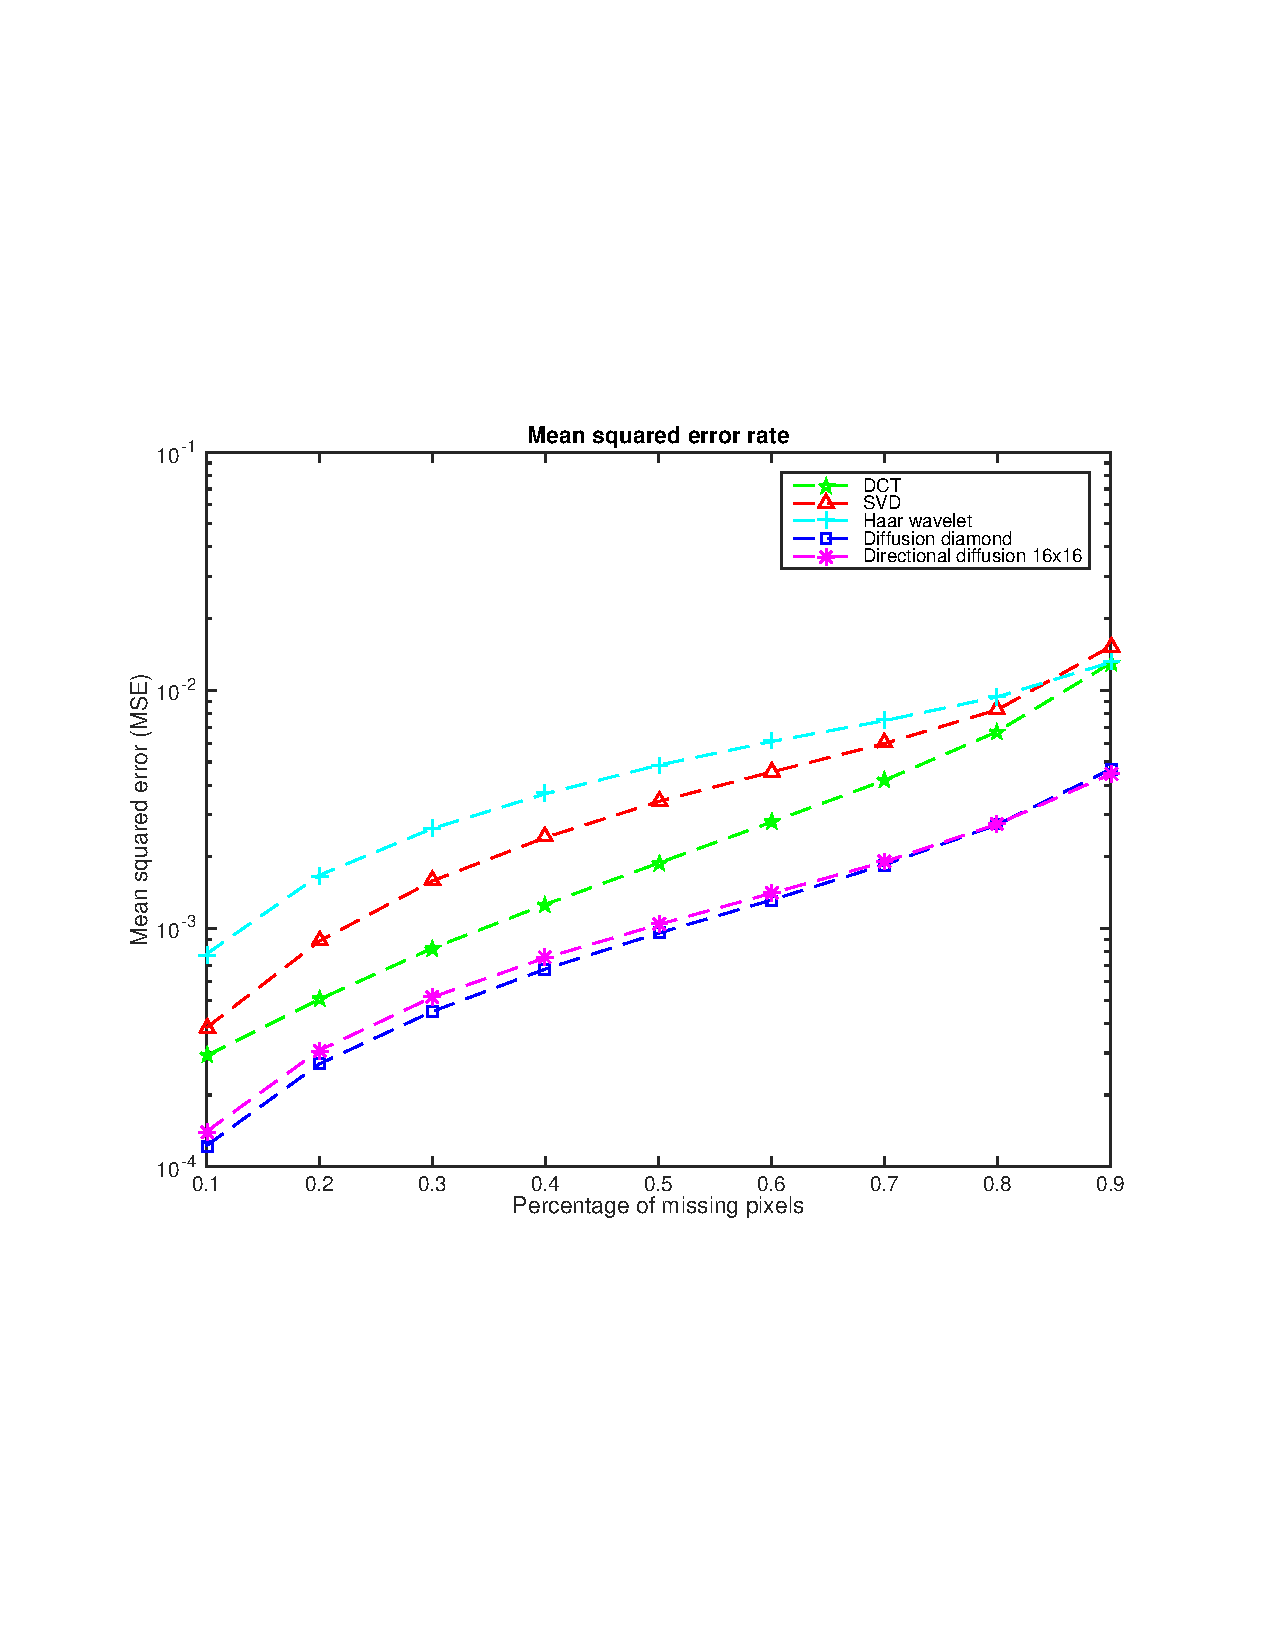
\includegraphics[clip, trim=2cm 7cm 2cm 6cm, width=0.9\textwidth]{figures/mse_vector}
		\caption{Mean squared error in log scale}
		\label{fig:err_random}
	\end{subfigure}
	\begin{subfigure}[b]{0.49\textwidth}
		\centering
		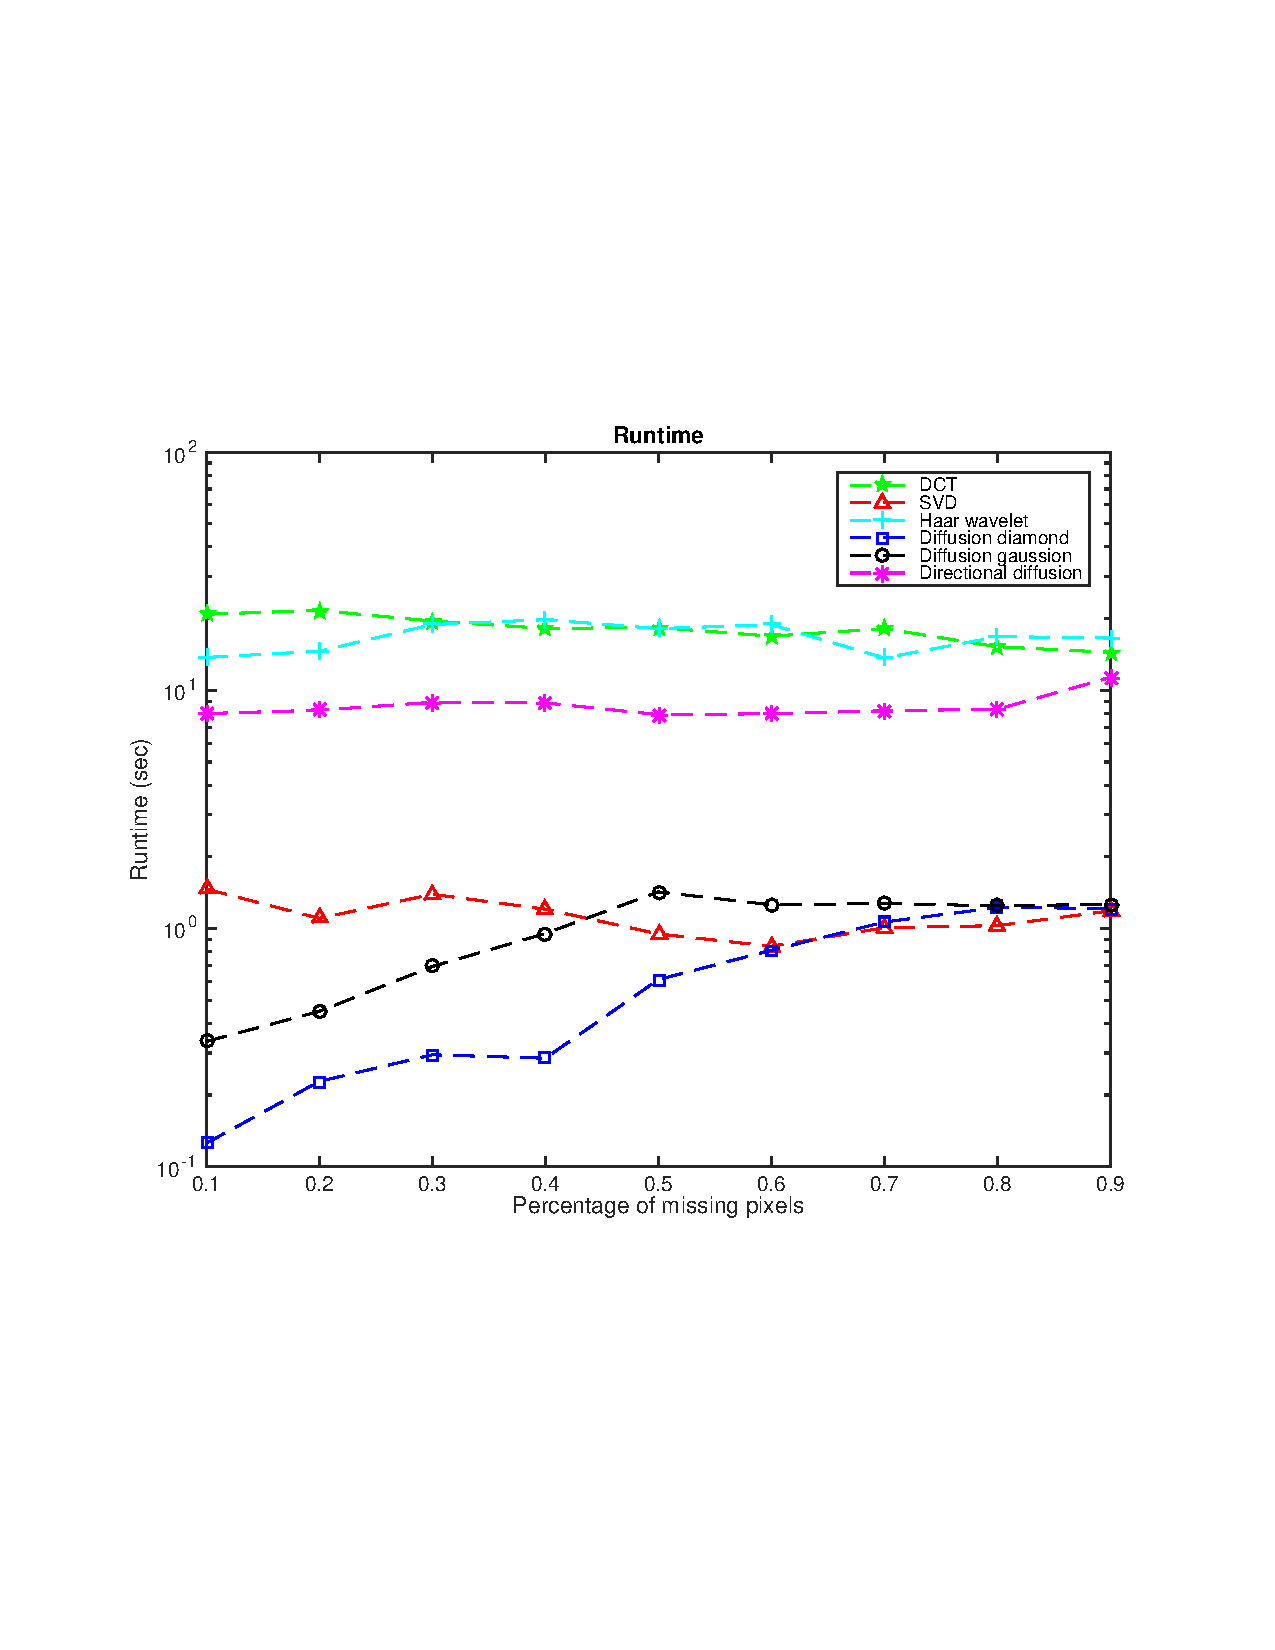
\includegraphics[clip, trim=2cm 7cm 2cm 6cm, width=0.9\textwidth]{figures/runtime_vector}
		\caption{Runtime in log scale}
		\label{fig:runtime}
	\end{subfigure}
	
	\caption{Mean squared error and runtime comparison with different algorithms}
	\label{fig:rmd_results}
\end{figure*}


Both the regular diffusion and the directional diffusion algorithm show promising results. From figure \ref{fig:err_random} we see that the regular diffusion algorithm with the $K_{\text{diamond}}$ kernel works best on a mask of randomly missing pixels. This can be explained by the fact that this algorithm diffuses nearby pixels into the missing regions. A mask with randomly missing pixels will, on average, have at least some pixels in the direct or near neighborhood of a pixel that we try to inpaint.

Table \ref{tbl:err_text} shows the mean squared error of the algorithms on a structured mask, namely a piece of text. The missing pixels have some structure and form medium-sized areas of missing pixels. The regular diffusion algorithm does not perform as well in this setting because it relies on nearby known pixels which are less common in masks with medium-sized areas of missing pixels. The high-contrasting edges of the underlying image are not properly extended into the unknown regions. The directional diffusion algorithm helps resolve this by aligning the kernel  $K_{\theta}$ with the general directionality of the image patches. Because of this the directional diffusion algorithm scores best. This does however come at the cost of a significant increase in runtime.

Although the directional diffusion scores slightly better than the regular diffusion algorithm on text masks, we feel the trade-off in execution time is not worth the increase in score. Hence we decided to submit the regular diffusion algorithm as a final submission to the scoreboard. In scenarios where the runtime is not a deciding factor, we would select the directional diffusion algorithm due to its lower mean squared error.